\section{Algorithm}
\label{sec:stereoroads}
We try to mitigate the $y$ resolution problems outlined in the previous section by also reducing the size of U,V roads and
 therefore the number of
accidental background hits in these roads. We use 12-strip U,V roads, also staggered by 8 strips, to avoid edge effects.
The algorithm uses 1-level U,V roads, one for each Micromegas stereo plane.
The X roads are still  4-level buffers collecting the hits of all X planes of the octuplet.
 The intersection of one U and one V road forms a  diamond, as
 illustrated by Fig.~\ref{fig:cartoon_smallroads_1}. 
 As shown in Fig.~\ref{fig:cartoon_smallroads_N}, many diamonds are needed to cover the full length of one X road.
%%%%%%%%%%%%%%%%%%%%%%%%%%%%%%%%%%%%%%%
\begin{figure}[!htpb]
  \begin{center}
    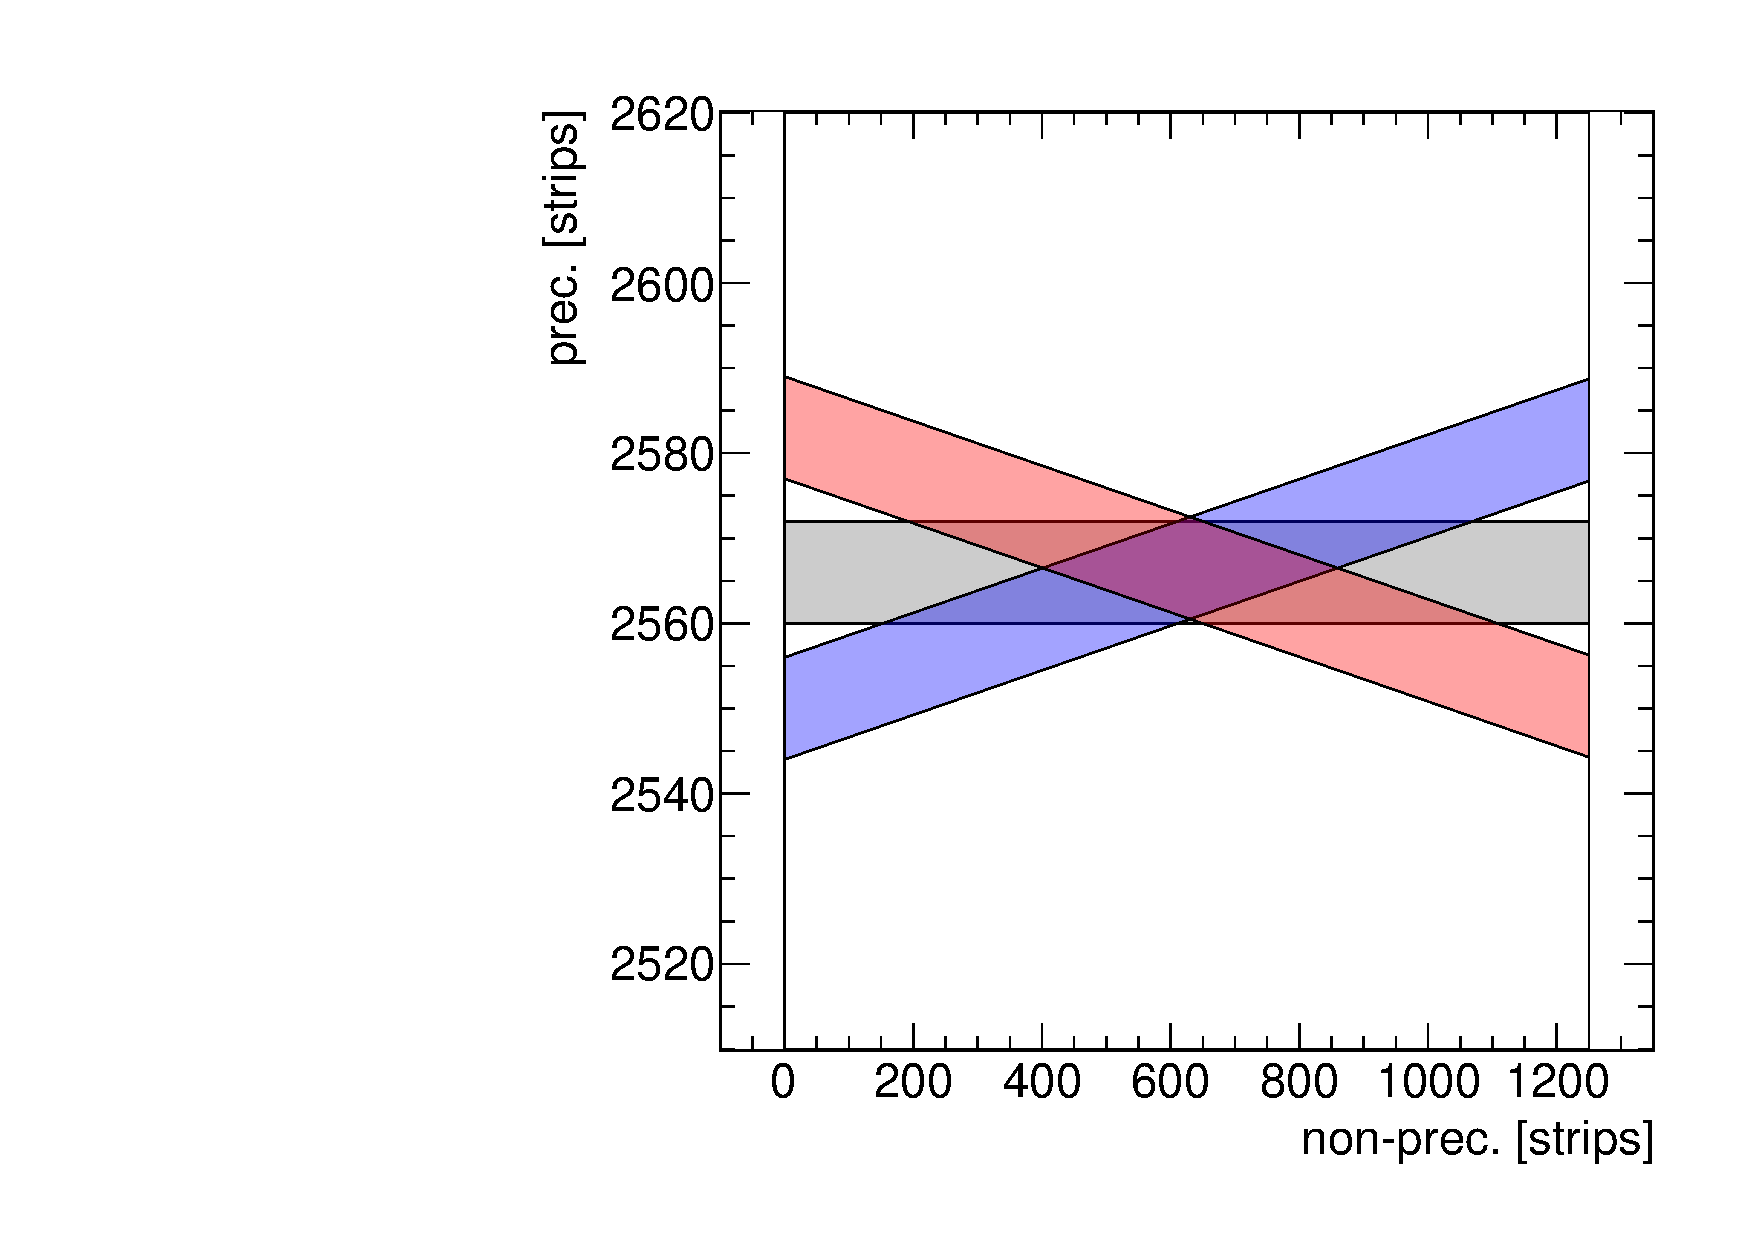
\includegraphics[width=0.48\textwidth]{figures/cartoon_roads_small_smallstereo_1.pdf}
    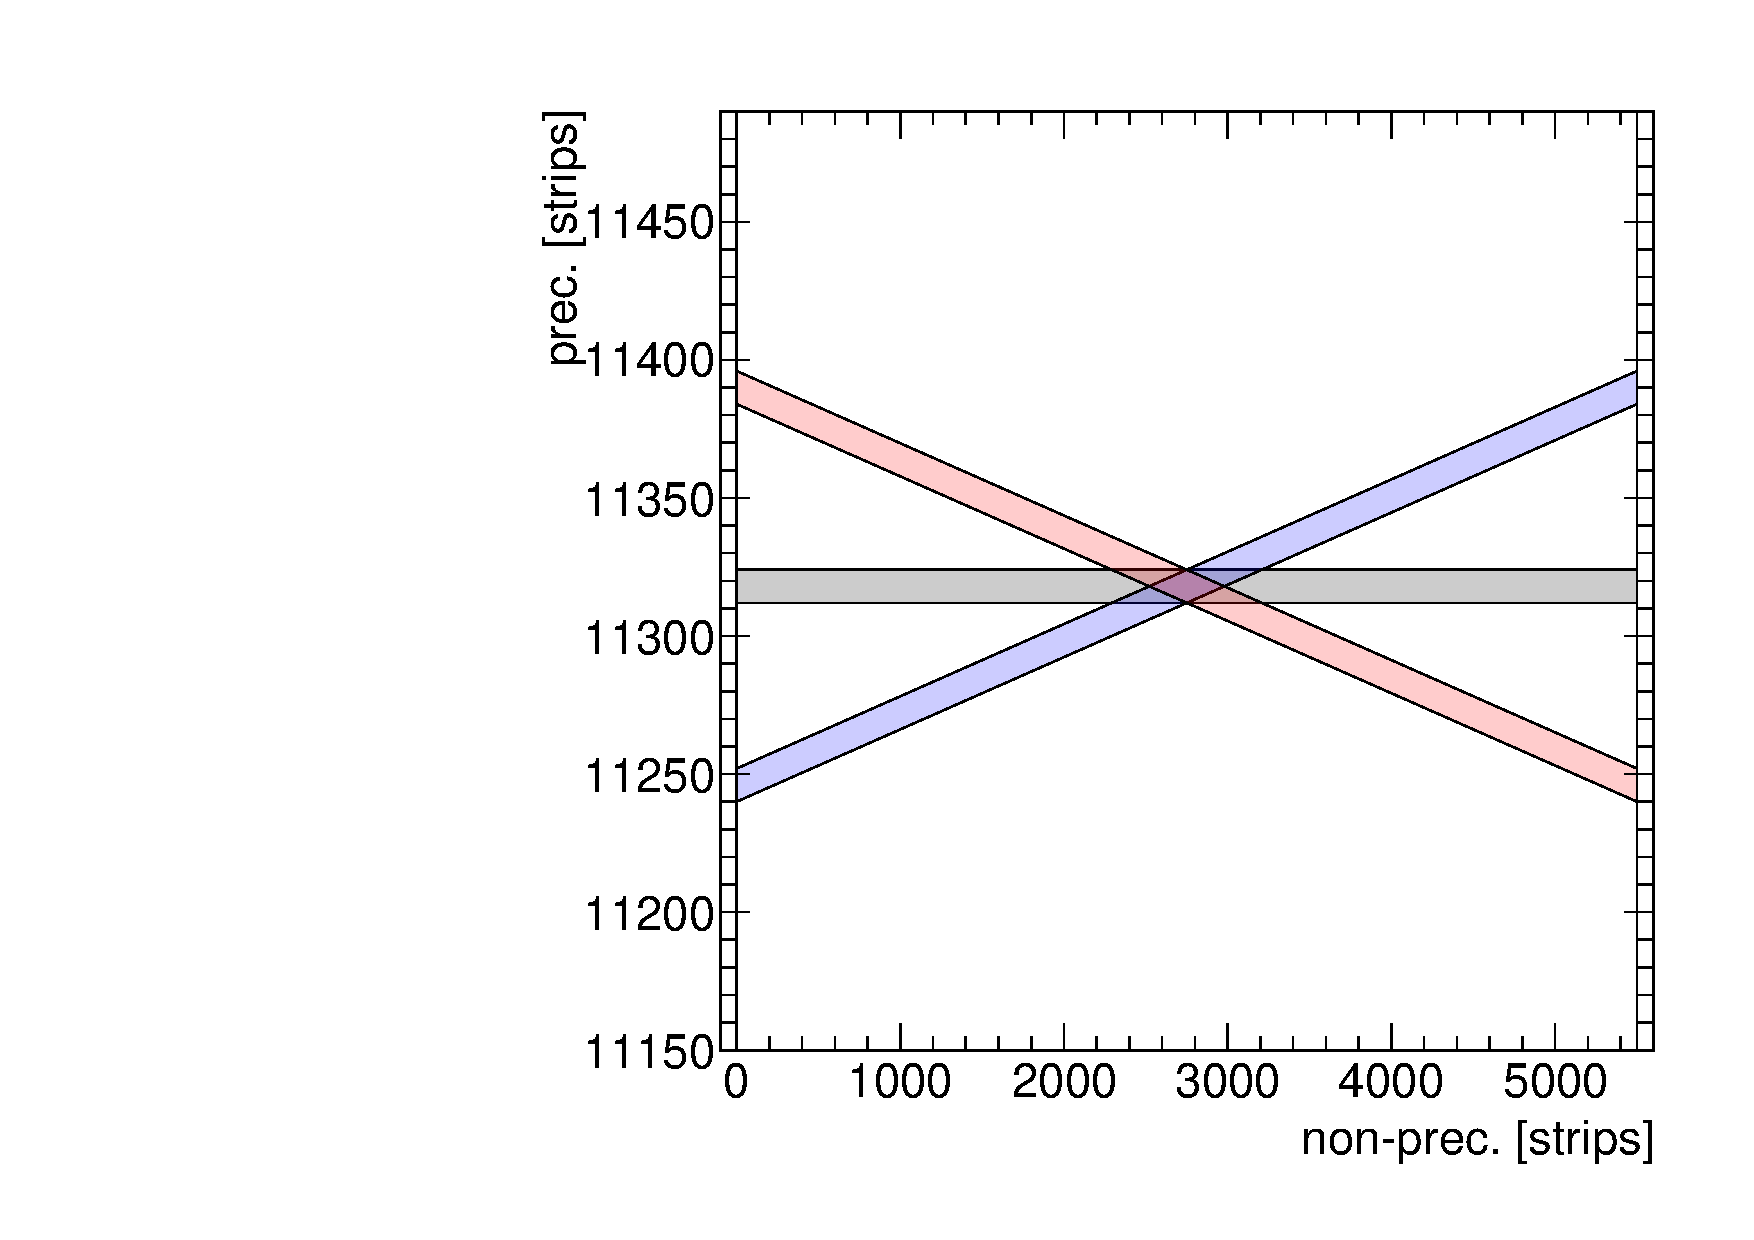
\includegraphics[width=0.48\textwidth]{figures/cartoon_roads_large_smallstereo_1.pdf}
  \end{center}
  \vspace{-10pt}
  \caption{Layout of the roads used by proposed MMTP algorithm, for a small chamber closest to the beamline (left)
 and large chamber farthest from the beamline (right). The X road is horizontal, the U road is pink and slanted,
 and the V road is blue and slanted. Only one pair of U and V roads is drawn, and  does not cover the entire length X road.
 The  $x$-axis (prec.) and $y$-axis (non-prec.) are in units of strip pitches, which are 0.4 mm.}
  \label{fig:cartoon_smallroads_1}
\end{figure}
%%%%%%%%%%%%%%%%%%%%%%%%%%%%%%%%%
%%%%%%%%%%%%%%%%%%%%%%%%%%%%%%%%%%
\begin{figure}[!htpb]
  \begin{center}
    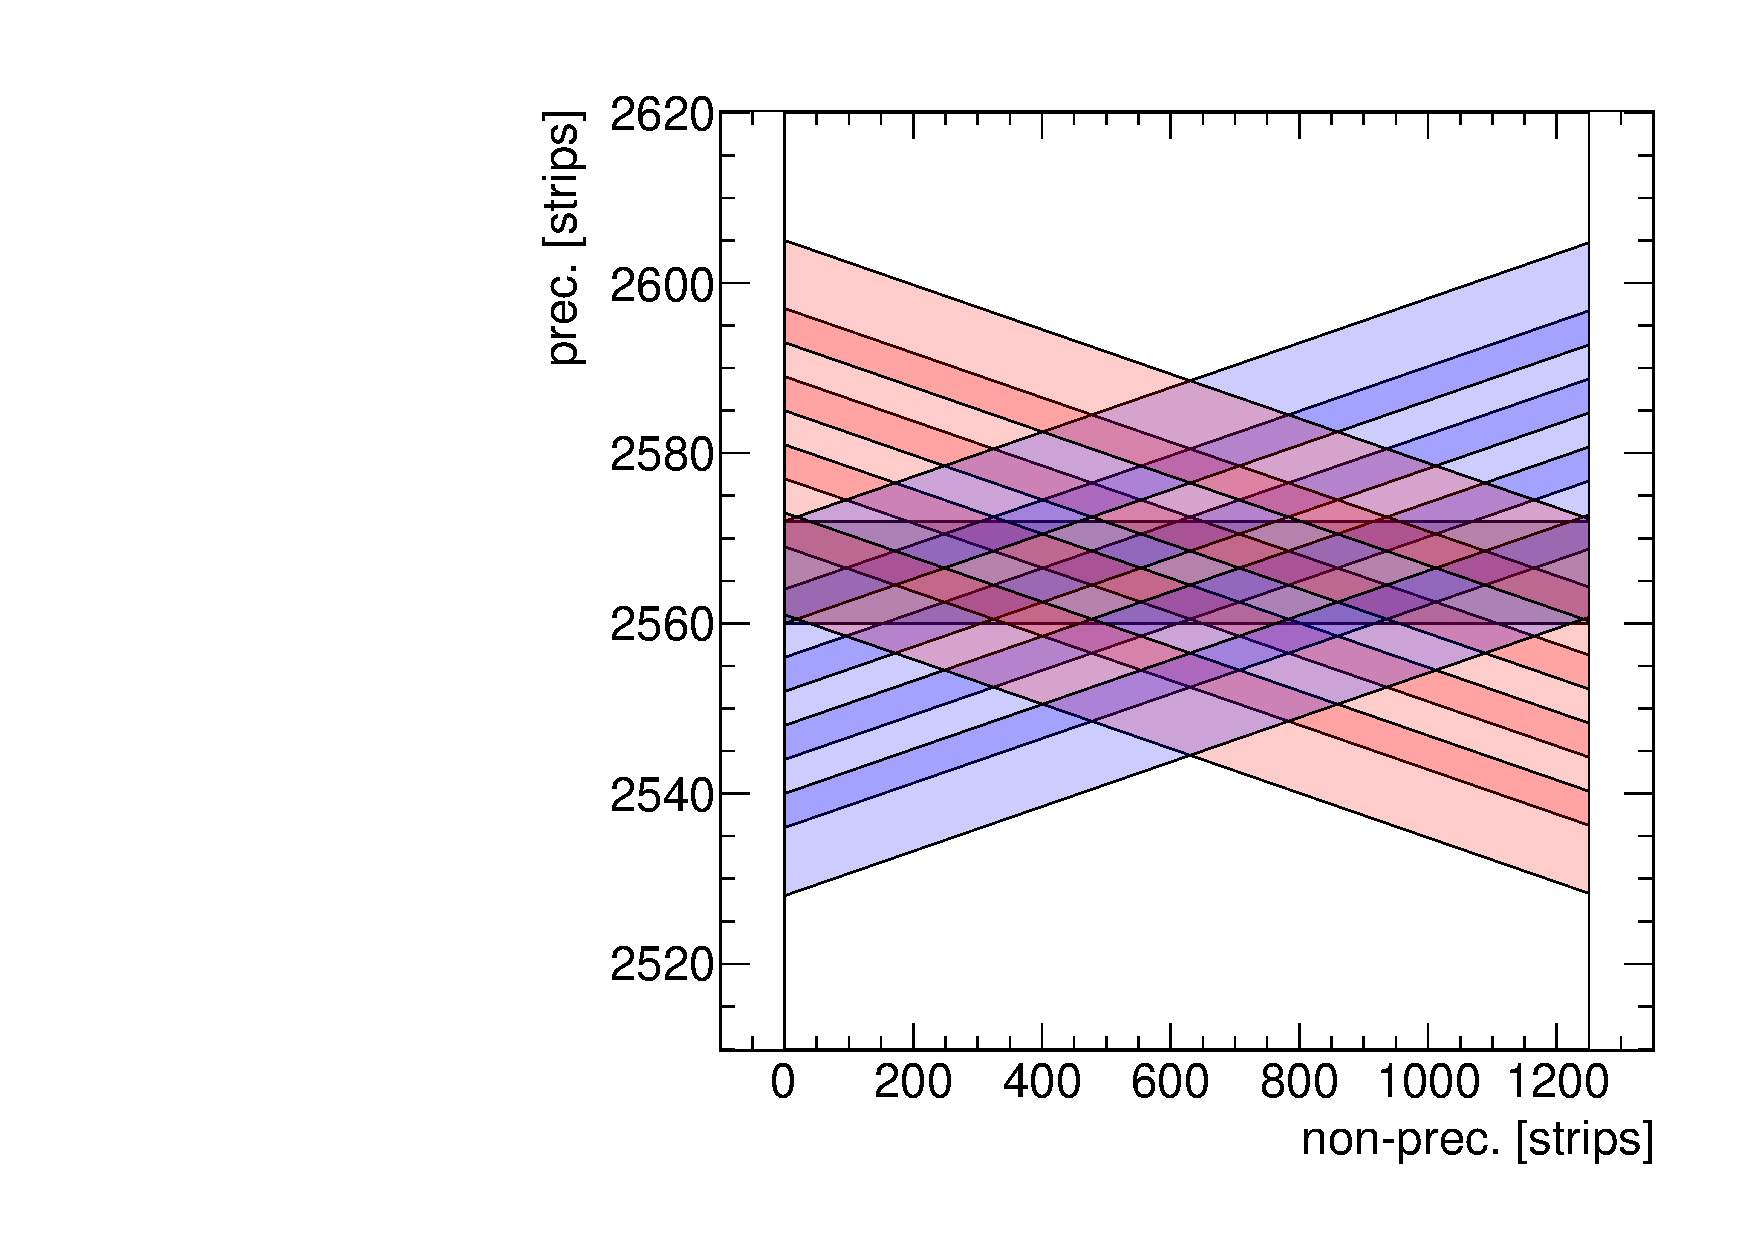
\includegraphics[width=0.48\textwidth]{figures/cartoon_roads_small_smallstereo_N.pdf}
    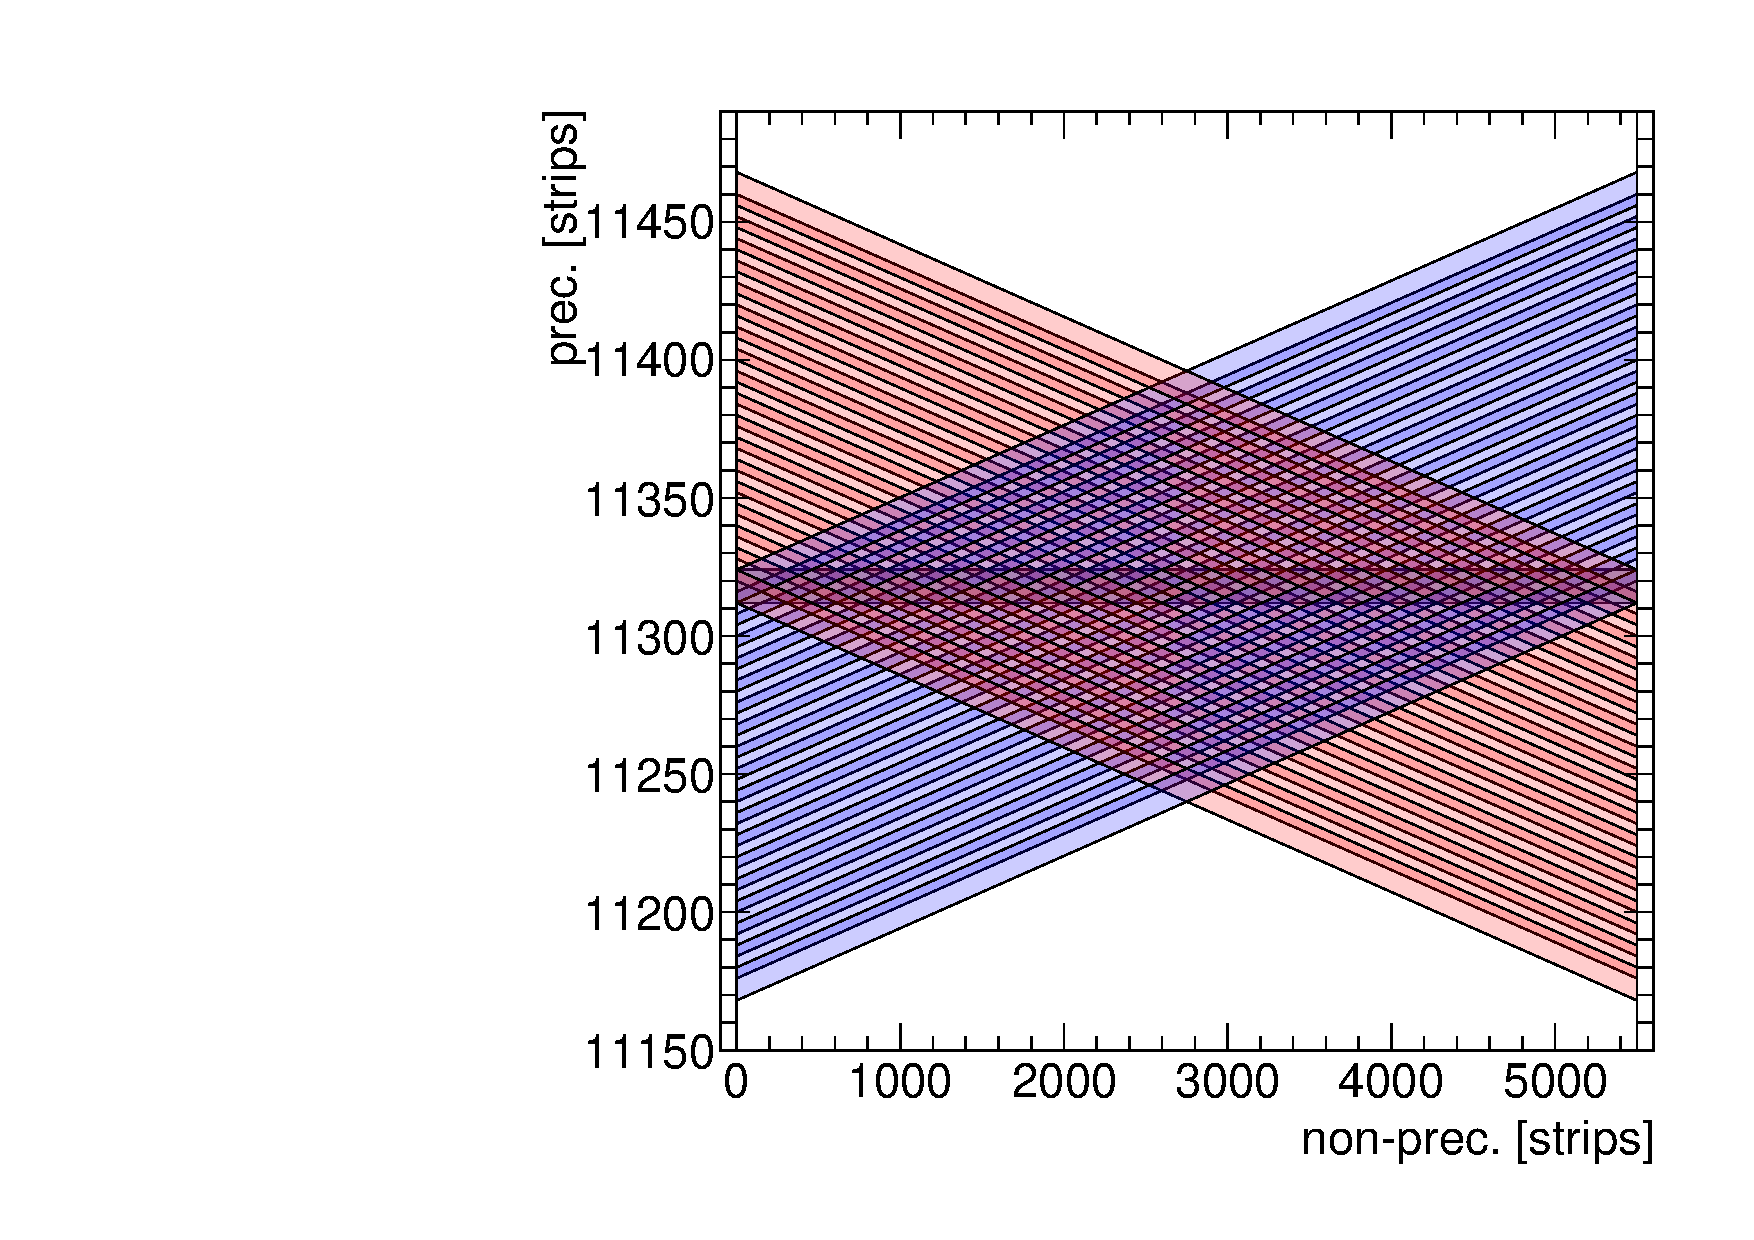
\includegraphics[width=0.48\textwidth]{figures/cartoon_roads_large_smallstereo_N.pdf}
  \end{center}
  \vspace{-10pt}
  \caption{Layout of the roads used by the proposed MMTP algorithm, for a small chamber closest to the beamline (left) and large chamber farthest
 from the beamline (right).The X road with shortest (longest) strips is covered with 5 (19) U and 5 (19) V roads.}
  \label{fig:cartoon_smallroads_N}
\end{figure}
%%%%%%%%%%%%%%%%%%%%%%%%%%%%%%%%%%%%%%%%%%%

 In the new algorithm, incoming hits are assigned to the respective X, U, and V roads with a maturity flag which expires after 8 (for now) BCs.  
 The  finder operates in two stages. In the first stage, the finder looks for any X road with at least 3 hits.
 If one such a road is found, in the second stage the finder enables a set of 4-fold majority AND-gates,
 one for each diamond overlapping the fired X road. The inputs
 of  each AND-gate corresponds to the four U,V roads defining the diamond and is set to 1 if a road has  one hit.
 If any of these coincidences has at least 3 U,V roads fired, a trigger is generated.
 This dramatically narrows the spatial region in which a coincidence is found.

\par The performance of the improved algorithm is illustrated by Figs.~\ref{fig:resolutions_new} and~\ref{fig:rms_vs_rate}. 
As expected, the $x$ resolution
 is comparable to that of the nominal algorithm that was already satisfactory. The $y$ resolution is much improved. 
Retaining as usual 99.7\% of the events, the rms value of the distribution is 11.22 (11.74) $\pm$ 0.01 (0.01) mm
 for 0.5 m (2.2 m) long strips.
%%%%%%%%%%%%%%%%%%%%%%%%%%%%%%%%%%%%%%%%%%%%%%%%%
\begin{figure}[!htpb]
  \begin{center}
    \includegraphics[width=0.48\textwidth]{figures/xres_new.pdf}
    \includegraphics[width=0.48\textwidth]{figures/yres_new.pdf}
    \includegraphics[width=0.48\textwidth]{figures/mres_new.pdf}
  \end{center}
  \vspace{-10pt}
  \caption{Distribution of $x_\text{reco.} - x_\text{truth}$ (top, left), $y_\text{reco.} - y_\text{truth}$ (top, right),
 and $\theta_\text{reco.} - \theta_\text{truth}$ (bottom)
 for the proposed MMTP algorithm in the presence of  uncorrelated background with a rate of 40 kHz per strip.
 This figure should be compared to Fig.~\ref{fig:resolutions_old}. }
  \label{fig:resolutions_new}
\end{figure}
%%%%%%%%%%%%%%%%%%%%%%%%%%%%%
%%%%%%%%%%%%%%%%%%%%%%%%%%%%
\begin{figure}[!htpb]
  \begin{center}
    \includegraphics[width=0.48\textwidth]{figures/rms_y_small_vs_rate.pdf}
    \includegraphics[width=0.48\textwidth]{figures/rms_y_large_vs_rate.pdf}
  \end{center}
  \vspace{-10pt}
  \caption{Dependence of rms value of $y_\text{reco.} - y_\text{truth}$  on
 the uncorrelated background rate for a strip length of (left) 0.5 m  and (right)  2.2 m.
 The rms is calculated  after a cut selecting 99\% of the events. This figure compares the performance of the nominal
and diamond-based algorithm.}
  \label{fig:rms_vs_rate}
\end{figure}
%%%%%%%%%%%%%%%%%%%%%%%%%%%%%%%%%%%%%%%%%%%%%
% We can also look at the efficiency of a $\Delta \phi <$ 20 mrad cut as a function of the uncorrelated background rate for both algorithms.
% In Figure \ref{fig:eff_vs_rate}, we see that the performance of the nominal algorithm drops sharply with increased background, 
%while the proposed algorithm maintains 80\% (95\%)+ efficiency for up to a 60 kHz/strip background rate with 0.5m (2.2m) long strips.
%\par We now elaborate on the use of implementation regions. It is important to divide the wedge into reasons so that each 
%implementation of the firmware has a minimum number of triggers to process at any given time. There will be hard limit to
% how many triggers can be processed per BC per implementation. Thus, small implementation regions are ideal. As a technical aside,
% the exact number of roads in an implementation region is presently determined by the architecture of
% the MMTP firmware. \footnote{The MMTP relies on multiplexers to select the $U$,$V$ roads overlapping with
% each $X$ road. If we consider the LM2 with a pitch of 450 microns,
% we have $2.2\text{m} \times \tan 1.5^\circ \times \frac{1}{450 \;\mu m \times 8 \text{ strips/road}} = 16 + 1$ $U$,$V$ roads associated
% to one $X$ road, so we need 17 multiplexers. Assuming standard multiplexer of 8:1, we can have 136 $X$ roads in the largest
% R region. A similar calculation can be done for the 0.5m strips.} 
%|begin{figure}[!htpb]
%  \begin{center}
%    \includegraphics[width=0.48\textwidth]{figures/eff_phi_small_vs_rate.pdf}
%    \includegraphics[width=0.48\textwidth]{figures/eff_phi_large_vs_rate.pdf}
%  \end{center}
%  \vspace{-10pt}
%  \caption{Efficiency of $\phi_\text{reco.} - \phi_\text{truth} < 20$ mrad for a strip size of 0.5m (left) and 2.2m (right).
% $\phi_\text{reco.}-\phi_\text{truth}$ is calculated as $\frac{y_\text{reco.} - y_\text{truth}}{R}$, where $R$ is the distance
% from the beamline. $R$ is taken to be 1m for the small chamber and 4.5m for the large chamber.}
%  \label{fig:eff_vs_rate}
%\end{figure}

